\documentclass[10pt,table,aspectratio=169]{beamer}

\usetheme[progressbar=frametitle]{metropolis}
\usepackage{appendixnumberbeamer}

\usepackage{booktabs}
\usepackage[scale=2]{ccicons}
\usepackage{media9}
\usepackage{multimedia}
\usetikzlibrary{positioning,arrows.meta,chains,fit, trees}
\usepackage{pgfplots}
\usepackage{soul}
\usepgfplotslibrary{dateplot}
\usepackage{multicol}
\usepackage{xspace}
\usepackage{setspace}
\usepackage{changepage}
\usepackage[export]{adjustbox}
\usepackage{subcaption}
\usepackage{wasysym}
\usepackage[10pt]{moresize}
\usepackage{ragged2e}
\usepackage{bigdelim}
\usepackage{fancyvrb}
\usepackage{tikz}
\usetikzlibrary{trees}

\usepackage{minted}

% Global options for minted
\setminted[r]{
  frame=single,
  fontsize=\scriptsize,
  breaklines,
  autogobble,
  label=R Code,
  style=tango, % Change the style as needed
}

\newcommand{\themename}{\textbf{\textsc{metropolis}}\xspace}
\setbeamertemplate{caption}{\raggedright\insertcaption\par}

\usepackage{tikz}
\usetikzlibrary{shapes,arrows,positioning,calc,arrows.meta}
\usetikzlibrary{decorations}
\usetikzlibrary{decorations.markings}
\usetikzlibrary{decorations.pathreplacing}

\usepackage{relsize}
\tikzset{fontscale/.style = {font=\relsize{#1}}
    }
\tikzset{>=latex}
\usetikzlibrary{shapes,arrows}

\usepackage{framed}

\newcommand{\fullframegraphic}[1]{
\begin{frame}
\includegraphics[height=\textheight,width=\textwidth,keepaspectratio]{#1}
\end{frame}
}


% conditional for xetex or luatex
\newif\ifxetexorluatex
\ifxetex
  \xetexorluatextrue
\else
  \ifluatex
    \xetexorluatextrue
  \else
    \xetexorluatexfalse
  \fi
\fi
%

\newcommand*\quotesize{50} % if quote size changes, need a way to make shifts relative
% Make commands for the quotes
\newcommand*{\openquote}
   {\tikz[remember picture,overlay,xshift=-3ex,yshift=-1.5ex]
   \node (OQ) {\quotefont\fontsize{\quotesize}{\quotesize}\selectfont``};\kern0pt}

\newcommand*{\closequote}[1]
  {\tikz[remember picture,overlay,xshift=2.5ex,yshift={#1}]
   \node (CQ) {\quotefont\fontsize{\quotesize}{\quotesize}\selectfont''};}

% select a colour for the shading
\colorlet{shadecolor}{white}

\newcommand*\shadedauthorformat{\emph} % define format for the author argument

% Now a command to allow left, right and centre alignment of the author
\newcommand*\authoralign[1]{%
  \if#1l
    \def\authorfill{}\def\quotefill{\hfill}
  \else
    \if#1r
      \def\authorfill{\hfill}\def\quotefill{}
    \else
      \if#1c
        \gdef\authorfill{\hfill}\def\quotefill{\hfill}
      \else\typeout{Invalid option}
      \fi
    \fi
  \fi}
% wrap everything in its own environment which takes one argument (author) and one optional argument
% specifying the alignment [l, r or c]
%
\newenvironment{shadequote}[2][l]%
{\authoralign{#1}
\ifblank{#2}
   {\def\shadequoteauthor{}\def\yshift{-2ex}\def\quotefill{\hfill}}
   {\def\shadequoteauthor{\par\authorfill\shadedauthorformat{#2}}\def\yshift{2ex}}
\begin{snugshade}\begin{quote}\openquote}
{\shadequoteauthor\quotefill\closequote{\yshift}\end{quote}\end{snugshade}}

\usepackage{soul}
\makeatletter
\let\HL\hl
\renewcommand\hl{%
  \let\set@color\beamerorig@set@color
  \let\reset@color\beamerorig@reset@color
  \HL}
\makeatother

\usepackage{scalerel}
\usepackage{xparse}



% \setlength{\leftmargini}{2pt}
\setbeamersize{text margin left=15pt,text margin right=15pt}
\setbeamercolor{background canvas}{bg=white}

\title{DML Applications}
\author{\vspace{-0.75em} Fanisi Mbozi, Gabrielle Péloquin-Skulski and Clemente Sánchez}
\date{\vspace{0.5em} Recent Developments in Political Methodology | September 29th, 2025}

\begin{document}

\maketitle


\setbeamertemplate{section in toc}[ball unnumbered]



\begin{frame}[plain, label = two_dimensions]{Advantages and Limitations of DML}

\begin{itemize}
    \item DML has the \alert{\bf advantage} of relaxing parametric assumptions.  
    \begin{itemize}
        \item Don't need to assume constant treatment effect
        \item Don't need to assume linearity \pause
    \end{itemize}
        \vspace{0.5em}
    \item DML has the \alert{\bf disadvantage} of assuming the \alert{\bf outcome model} and the \alert{\bf propensity score model}. \pause
        \vspace{0.5em}
    \item \alert{\bf Experimental design}: treatment is random, so the propensity score is known and bias is minimized \pause
        \vspace{0.5em}
    \item \alert{\bf Observational design}: bias can arise from misspecification of either model 
\end{itemize}
\end{frame}

\begin{frame}[plain, label = two_dimensions]{Causal Model Choice}
\centering
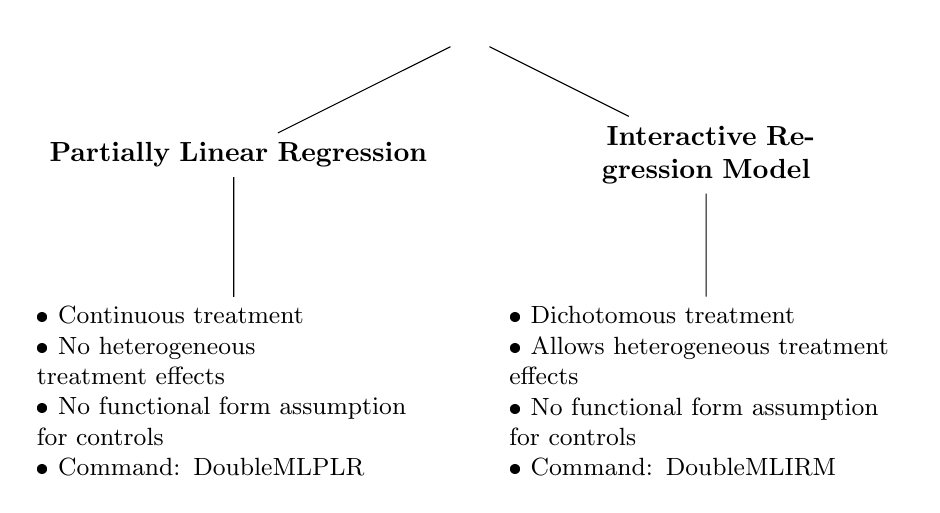
\begin{tikzpicture}[
  level 1/.style={sibling distance=6cm, level distance=1.5cm},
  level 2/.style={sibling distance=3cm, level distance=3cm},
  every node/.style={align=center, text width=5cm}
]

% Root
\node {}
  % Left branch
  child  {node (A) {\alert{ \bf Partially Linear Regression}} 
    child {node  [align=left, font=\small]  {• Continuous treatment \\ • No heterogeneous \\ treatment effects \\ • No functional form assumption for controls \\ • Command: DoubleMLPLR}}
  }
  % Right branch
  child {node (B) {\alert{ \bf Interactive Regression Model}}
    child {node [align=left, font=\small] {• Dichotomous treatment \\ • Allows heterogeneous treatment effects \\ • No functional form assumption for controls  \\ • Command: DoubleMLIRM}}
  };

\end{tikzpicture}
\pause
\begin{itemize}
  \item \alert{\bf Clustered Data:} DML assumes i.i.d.; assign whole clusters to folds and use cluster-robust SEs (Command: DoubleMLClusterData). 

\end{itemize}
\end{frame}

\section{Experimental design}

\begin{frame}[plain, label = two_dimensions]{Platas and Raffler (2021)}

Experiment on the effects of providing information in dominant party regimes. 
\begin{itemize}
  \item Information asymmetry in dominant party regimes. 
  \item Can provision of information about all parties: increase voter knowledge, improve opposition likability or alter vote intentions. 
  \item  11 constituencies in Uganda, within constituency randomly assign some villages to a screening of parliamentary candidate debates. 
\end{itemize}

\end{frame}


\begin{frame}[plain, label = two_dimensions]{Replicating original results}

\end{frame}


\begin{frame}[plain, label = two_dimensions]{DML application for experiment}

\end{frame}


\section{Observational design}

\begin{frame}[plain, label = two_dimensions]{Brierley and Nathan (2022)}

Motivating the Machine: Which Brokers do Parties Pay?

\begin{itemize}
  \item How do elites compensate brokers for their help during elections?
  \item While some might act due to ideological commitments, the literature suggests that most of them require material incentives.
  \item Little evidence of compensation by the literature, and what little there is focuses exclusively in the campaign season.
  \item \textit{Immediately after the election elites reward brokers that have delivered votes, but later on they reward brokers with connections.}
\end{itemize}

Design

\begin{itemize}
  \item Survey of 1,000 party brokers in Ghana.
  \item Condition on observables.
\end{itemize}

\end{frame}


\begin{frame}[plain, label = two_dimensions]{Replicating original results}

Main relationship:

\begin{itemize}
  \item T5: Payment immediately after election $\sim$ Vote swing
  \item T6: Payment after two years $\sim$ Number of connections
\end{itemize}

Additional:

\begin{itemize}
  \item Matrix of covariates
  \item Constituency fixed effects
  \item SEs clustered at the polling station
\end{itemize}

\begin{figure}[H]
    \centering
    \begin{subfigure}{0.4\textwidth}
        \centering
        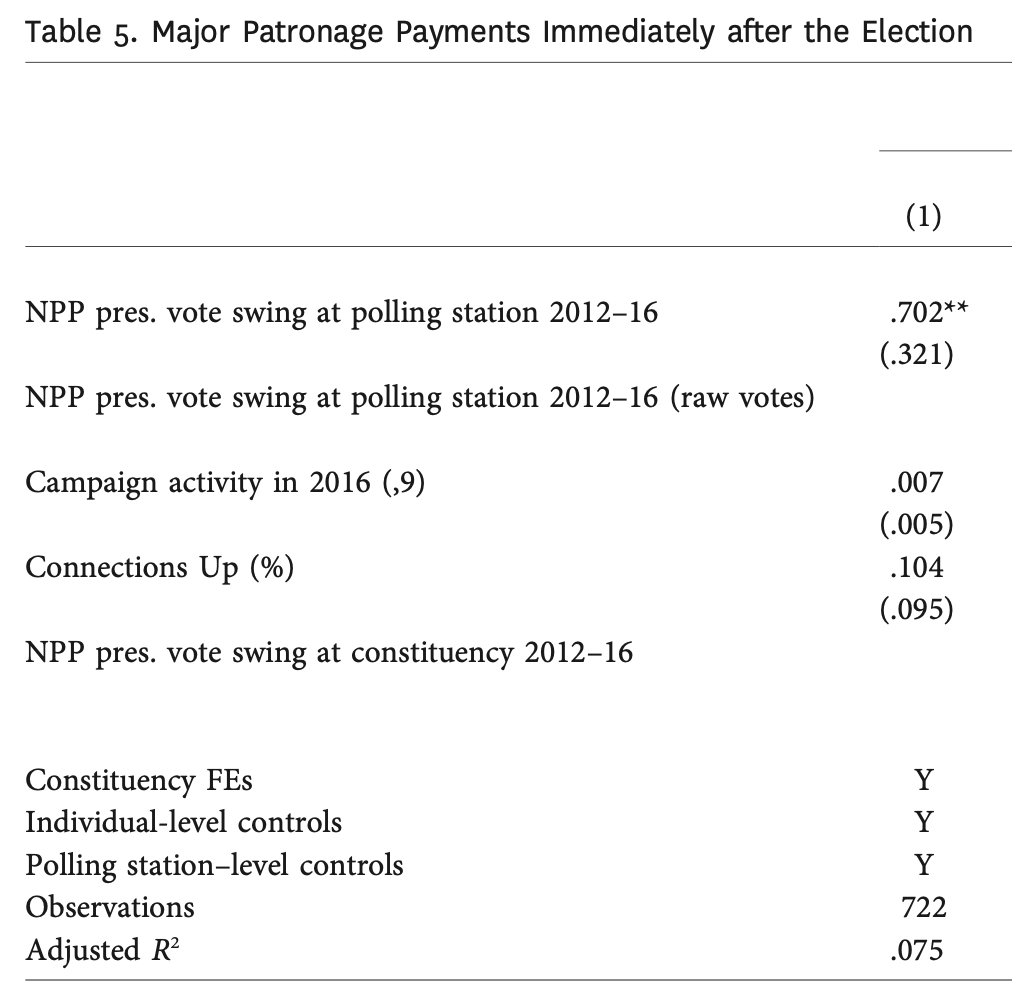
\includegraphics[width=\linewidth]{figures/observational_replication_t5.png}
    \end{subfigure}
    \hfill
    \begin{subfigure}{0.2\textwidth}
        \centering
        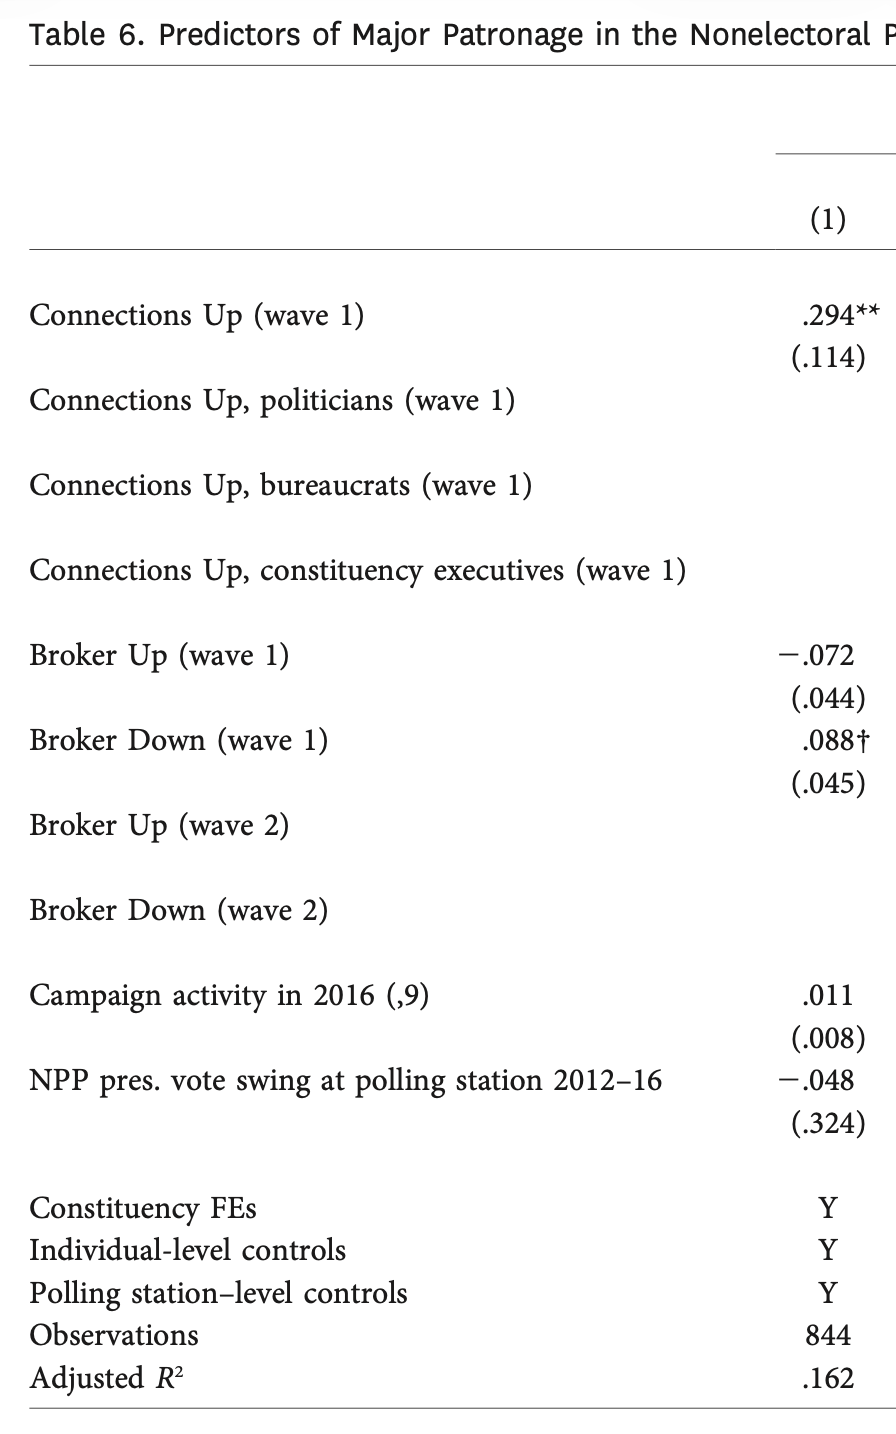
\includegraphics[width=\linewidth]{figures/observational_replication_t6.png}
    \end{subfigure}
    \hfill
    \begin{subfigure}{0.3\textwidth}
        \centering
        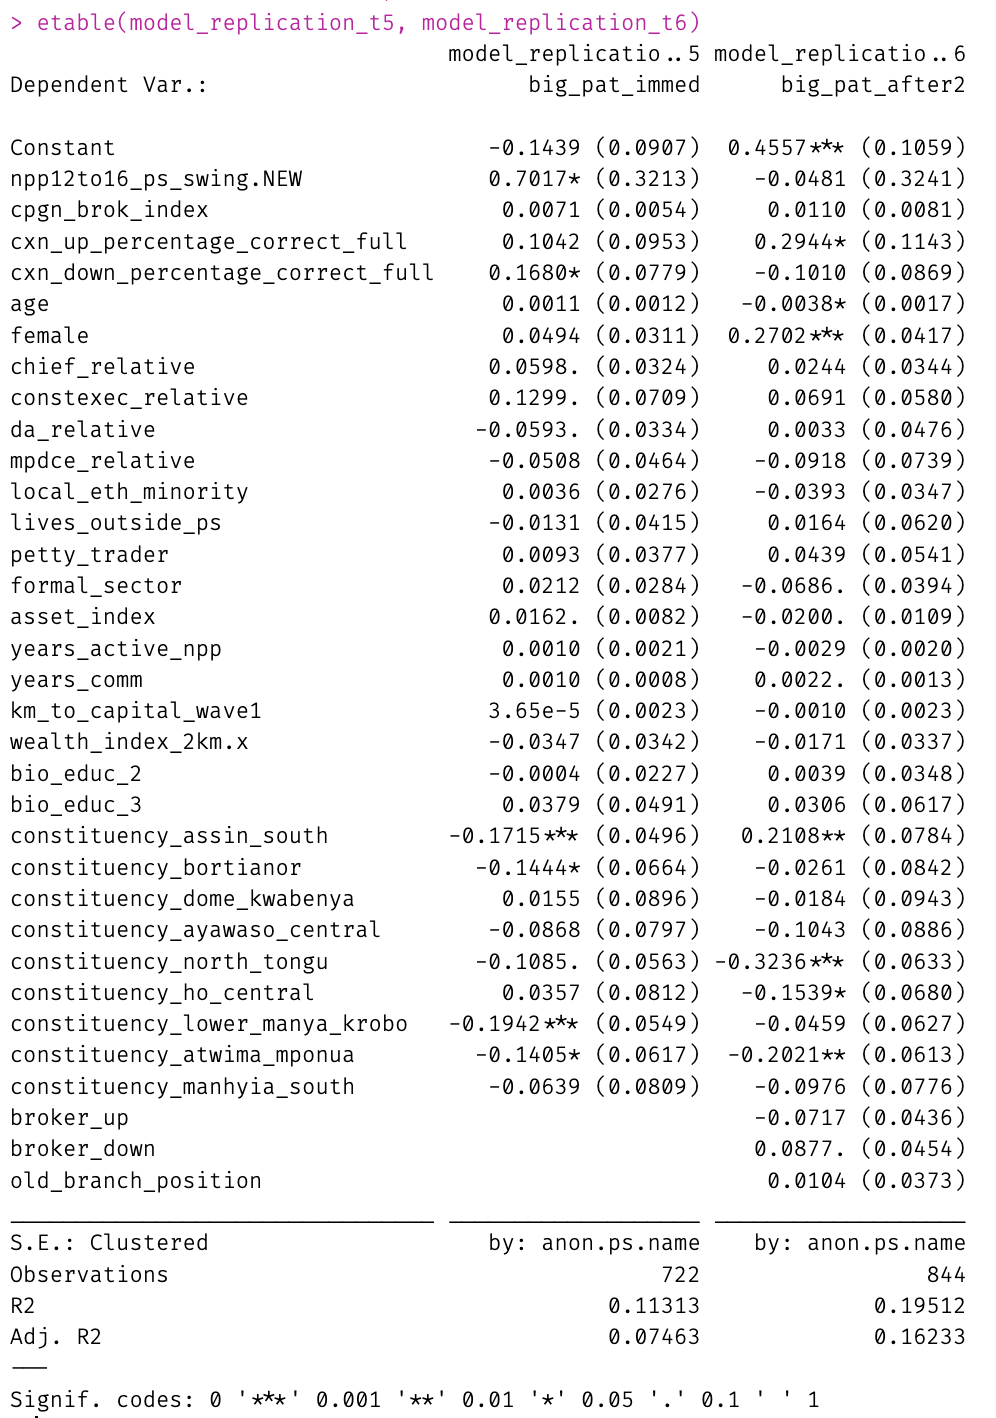
\includegraphics[width=\linewidth]{figures/observational_replication_feols.png}
    \end{subfigure}
\end{figure}

\end{frame}


\begin{frame}[plain, label = two_dimensions]{DML application for observational study}

Five-fold cross-fitting and 20 repetitions

\begin{figure}[H]
  \centering
  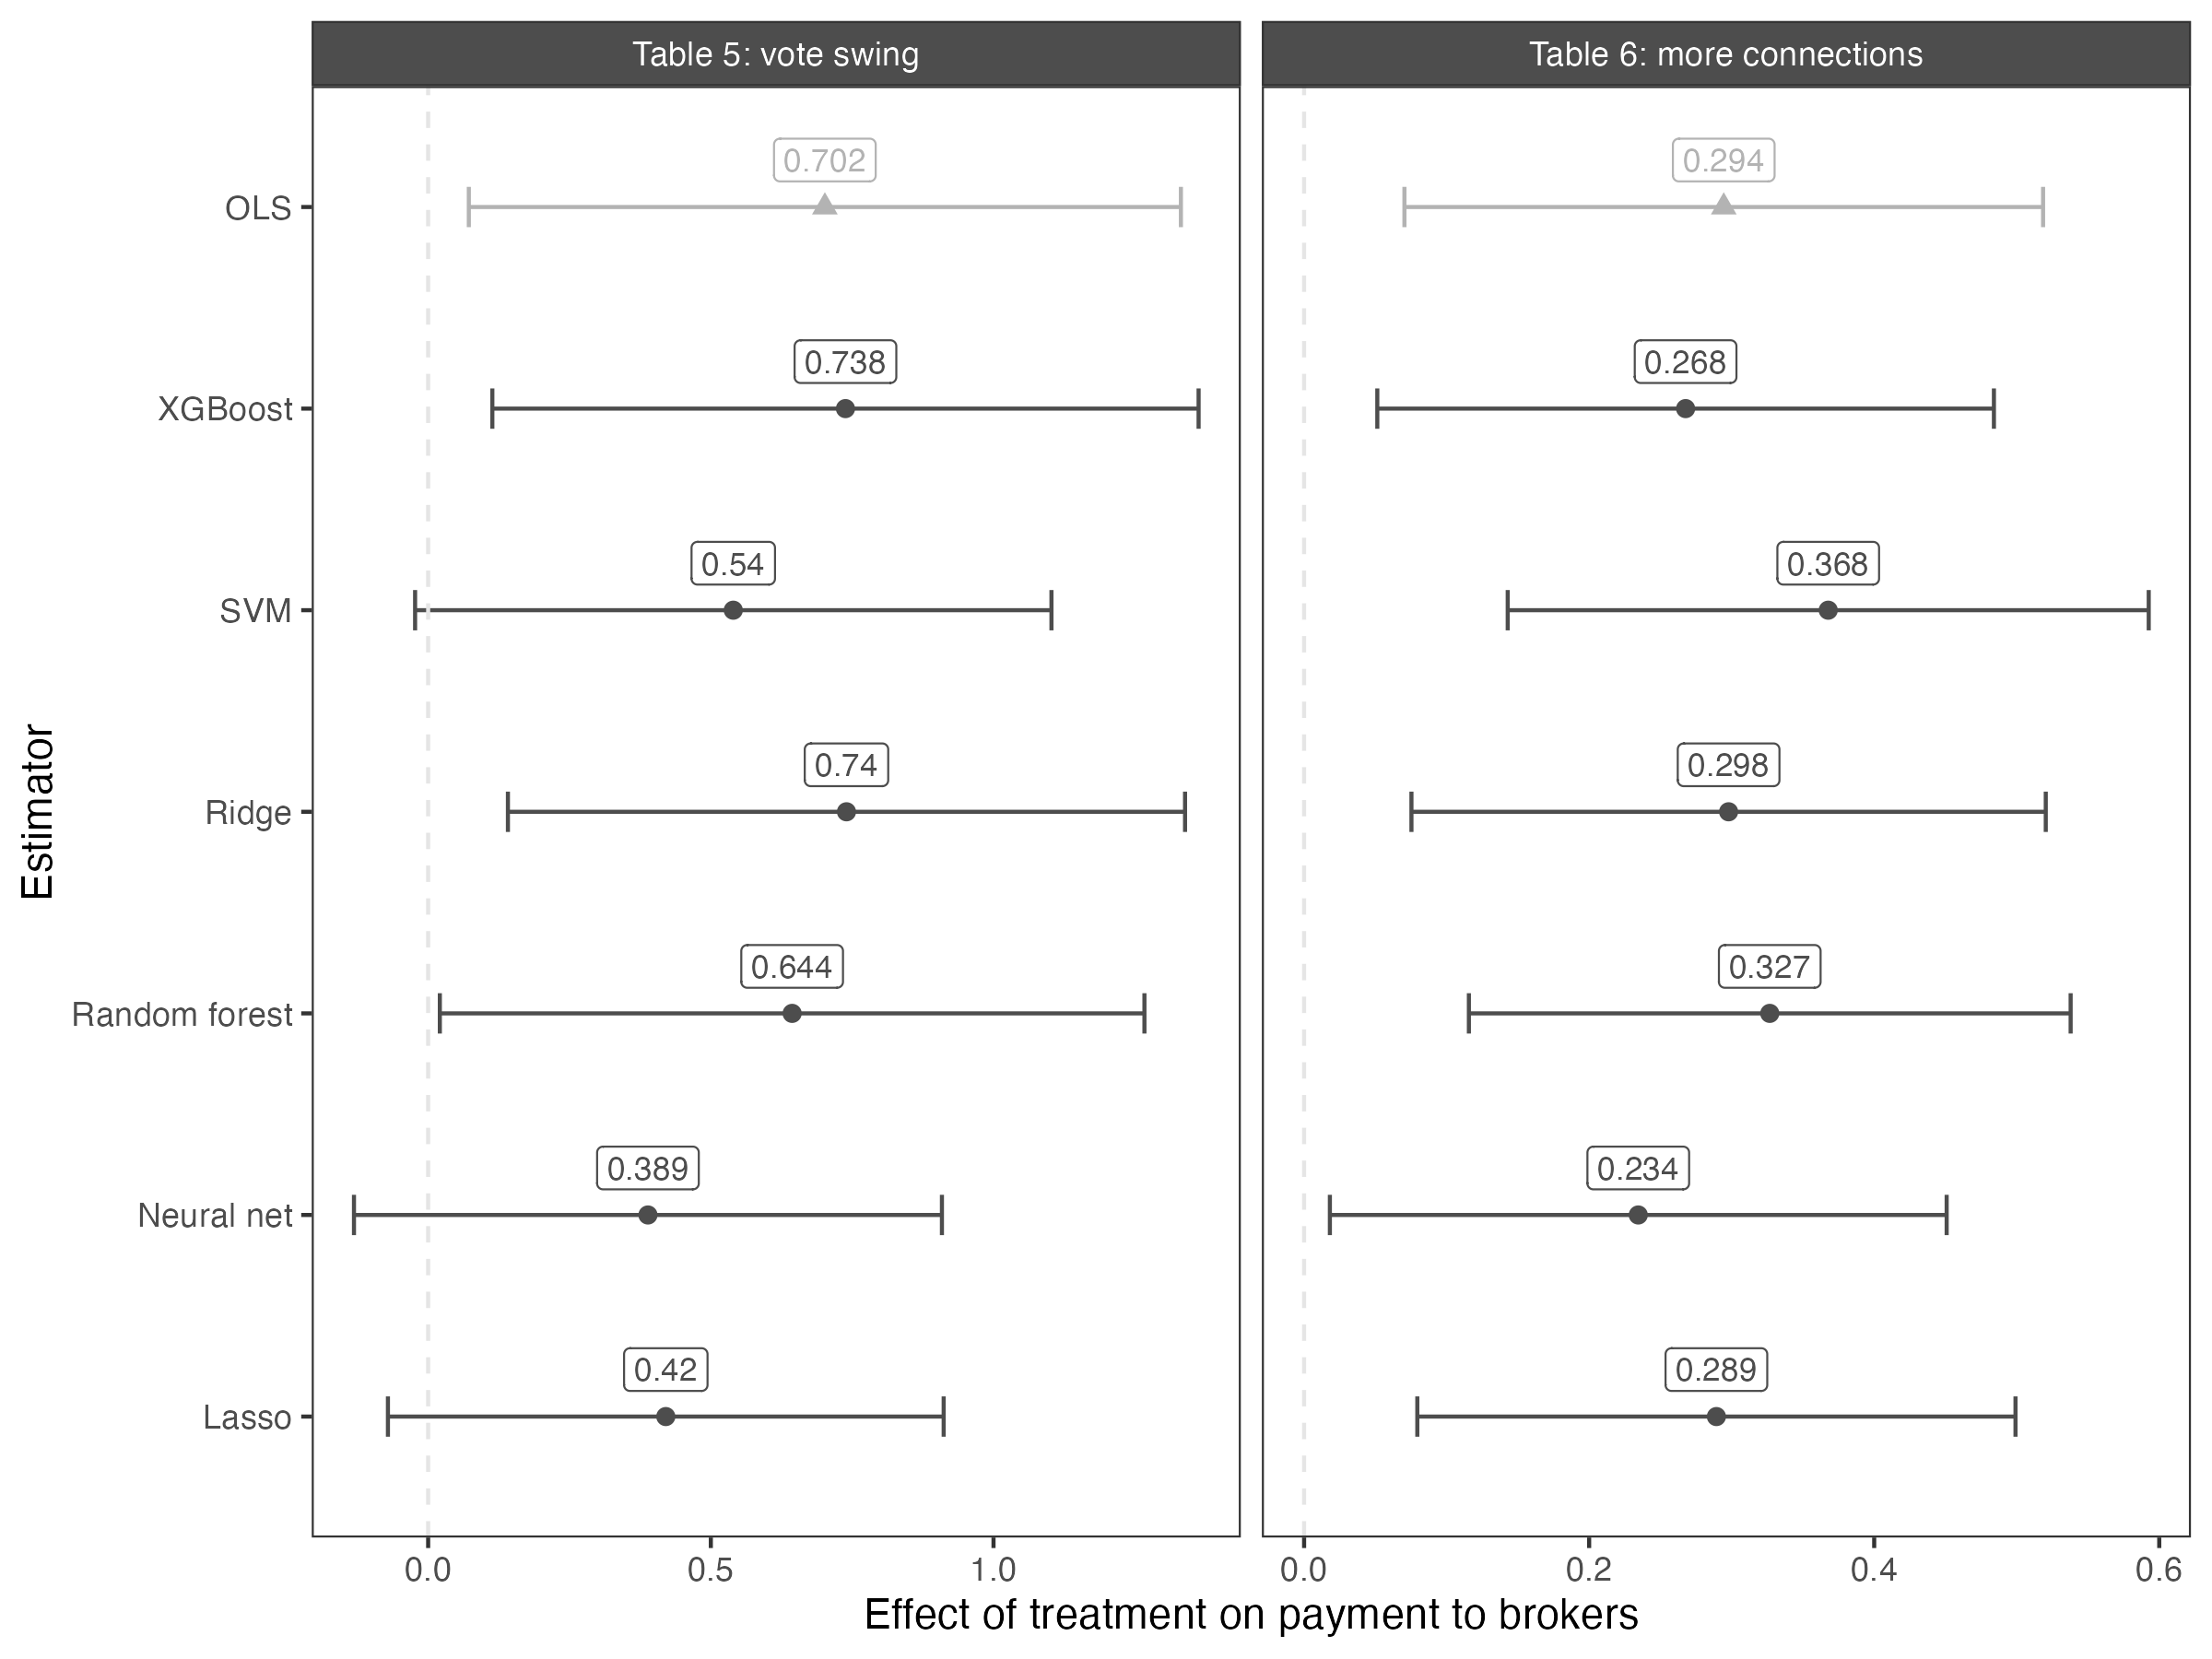
\includegraphics[height=0.9\textheight]{figures/observational_coefplot_dml.png}
\end{figure}
\end{frame}


\begin{frame}[plain, label = two_dimensions]{Balance of covariates}

\begin{figure}[H]
 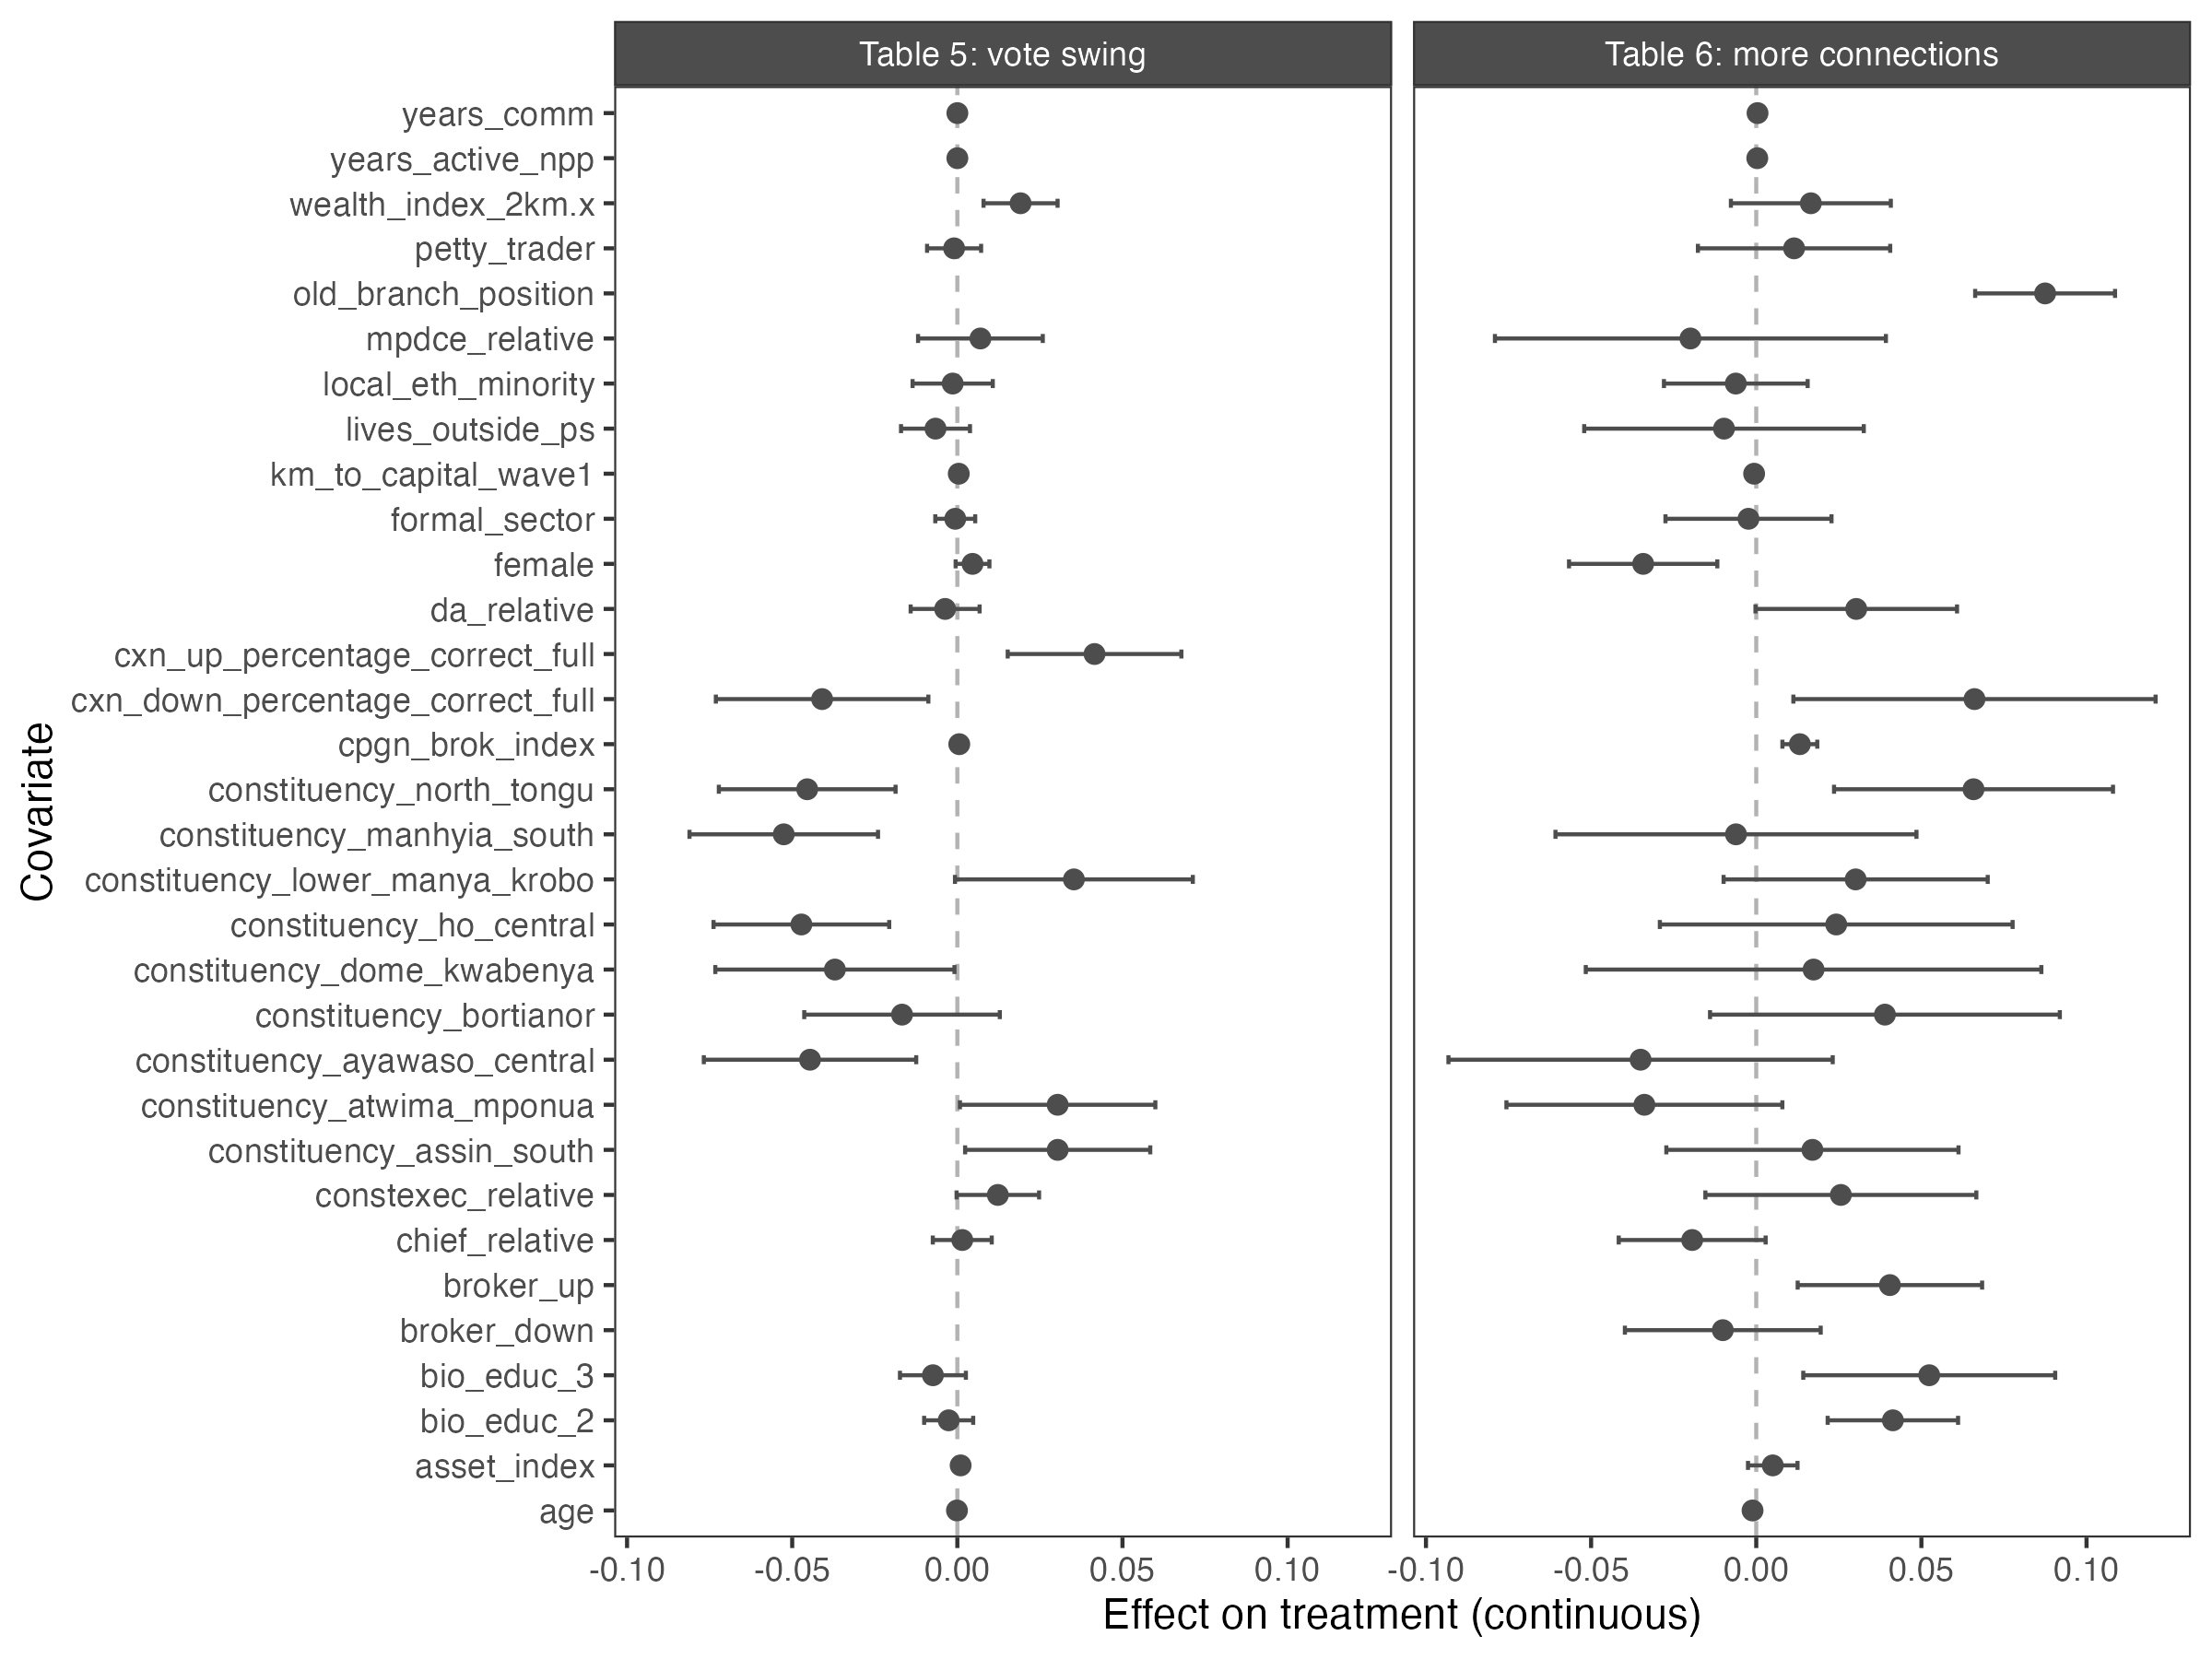
\includegraphics[height=0.9\textheight]{figures/observational_coefplot_balance.png}
\end{figure}

\end{frame}


\begin{frame}[plain, label = two_dimensions]{General propensity approach}

\begin{figure}[H]
 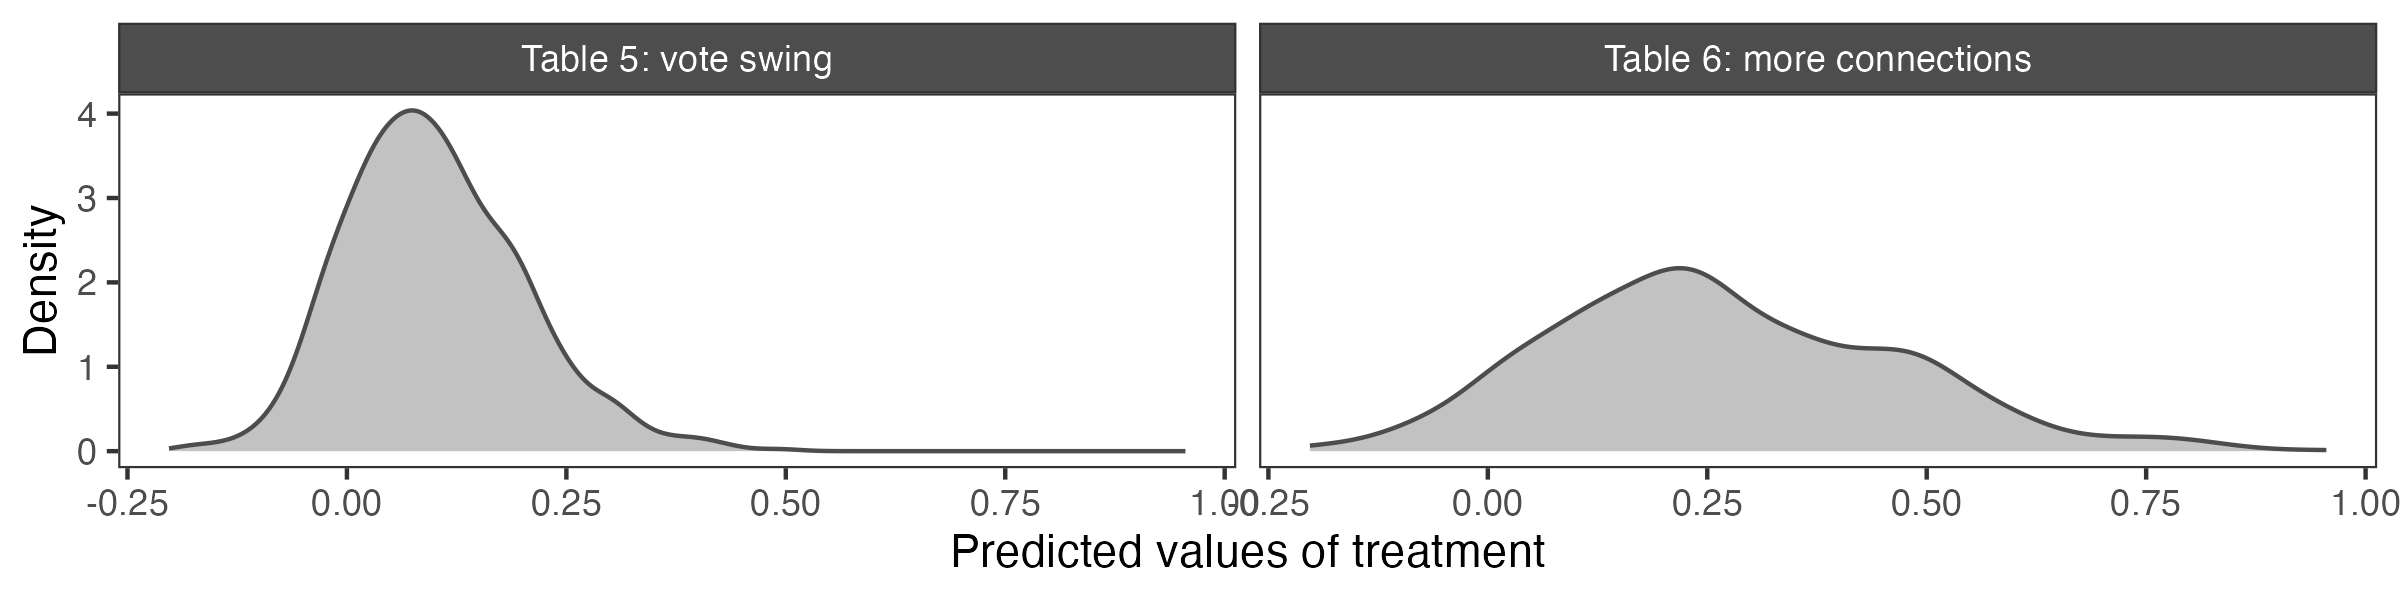
\includegraphics[width=0.7\linewidth]{figures/observational_density_predicted.png}
\end{figure}
\begin{figure}[H]
 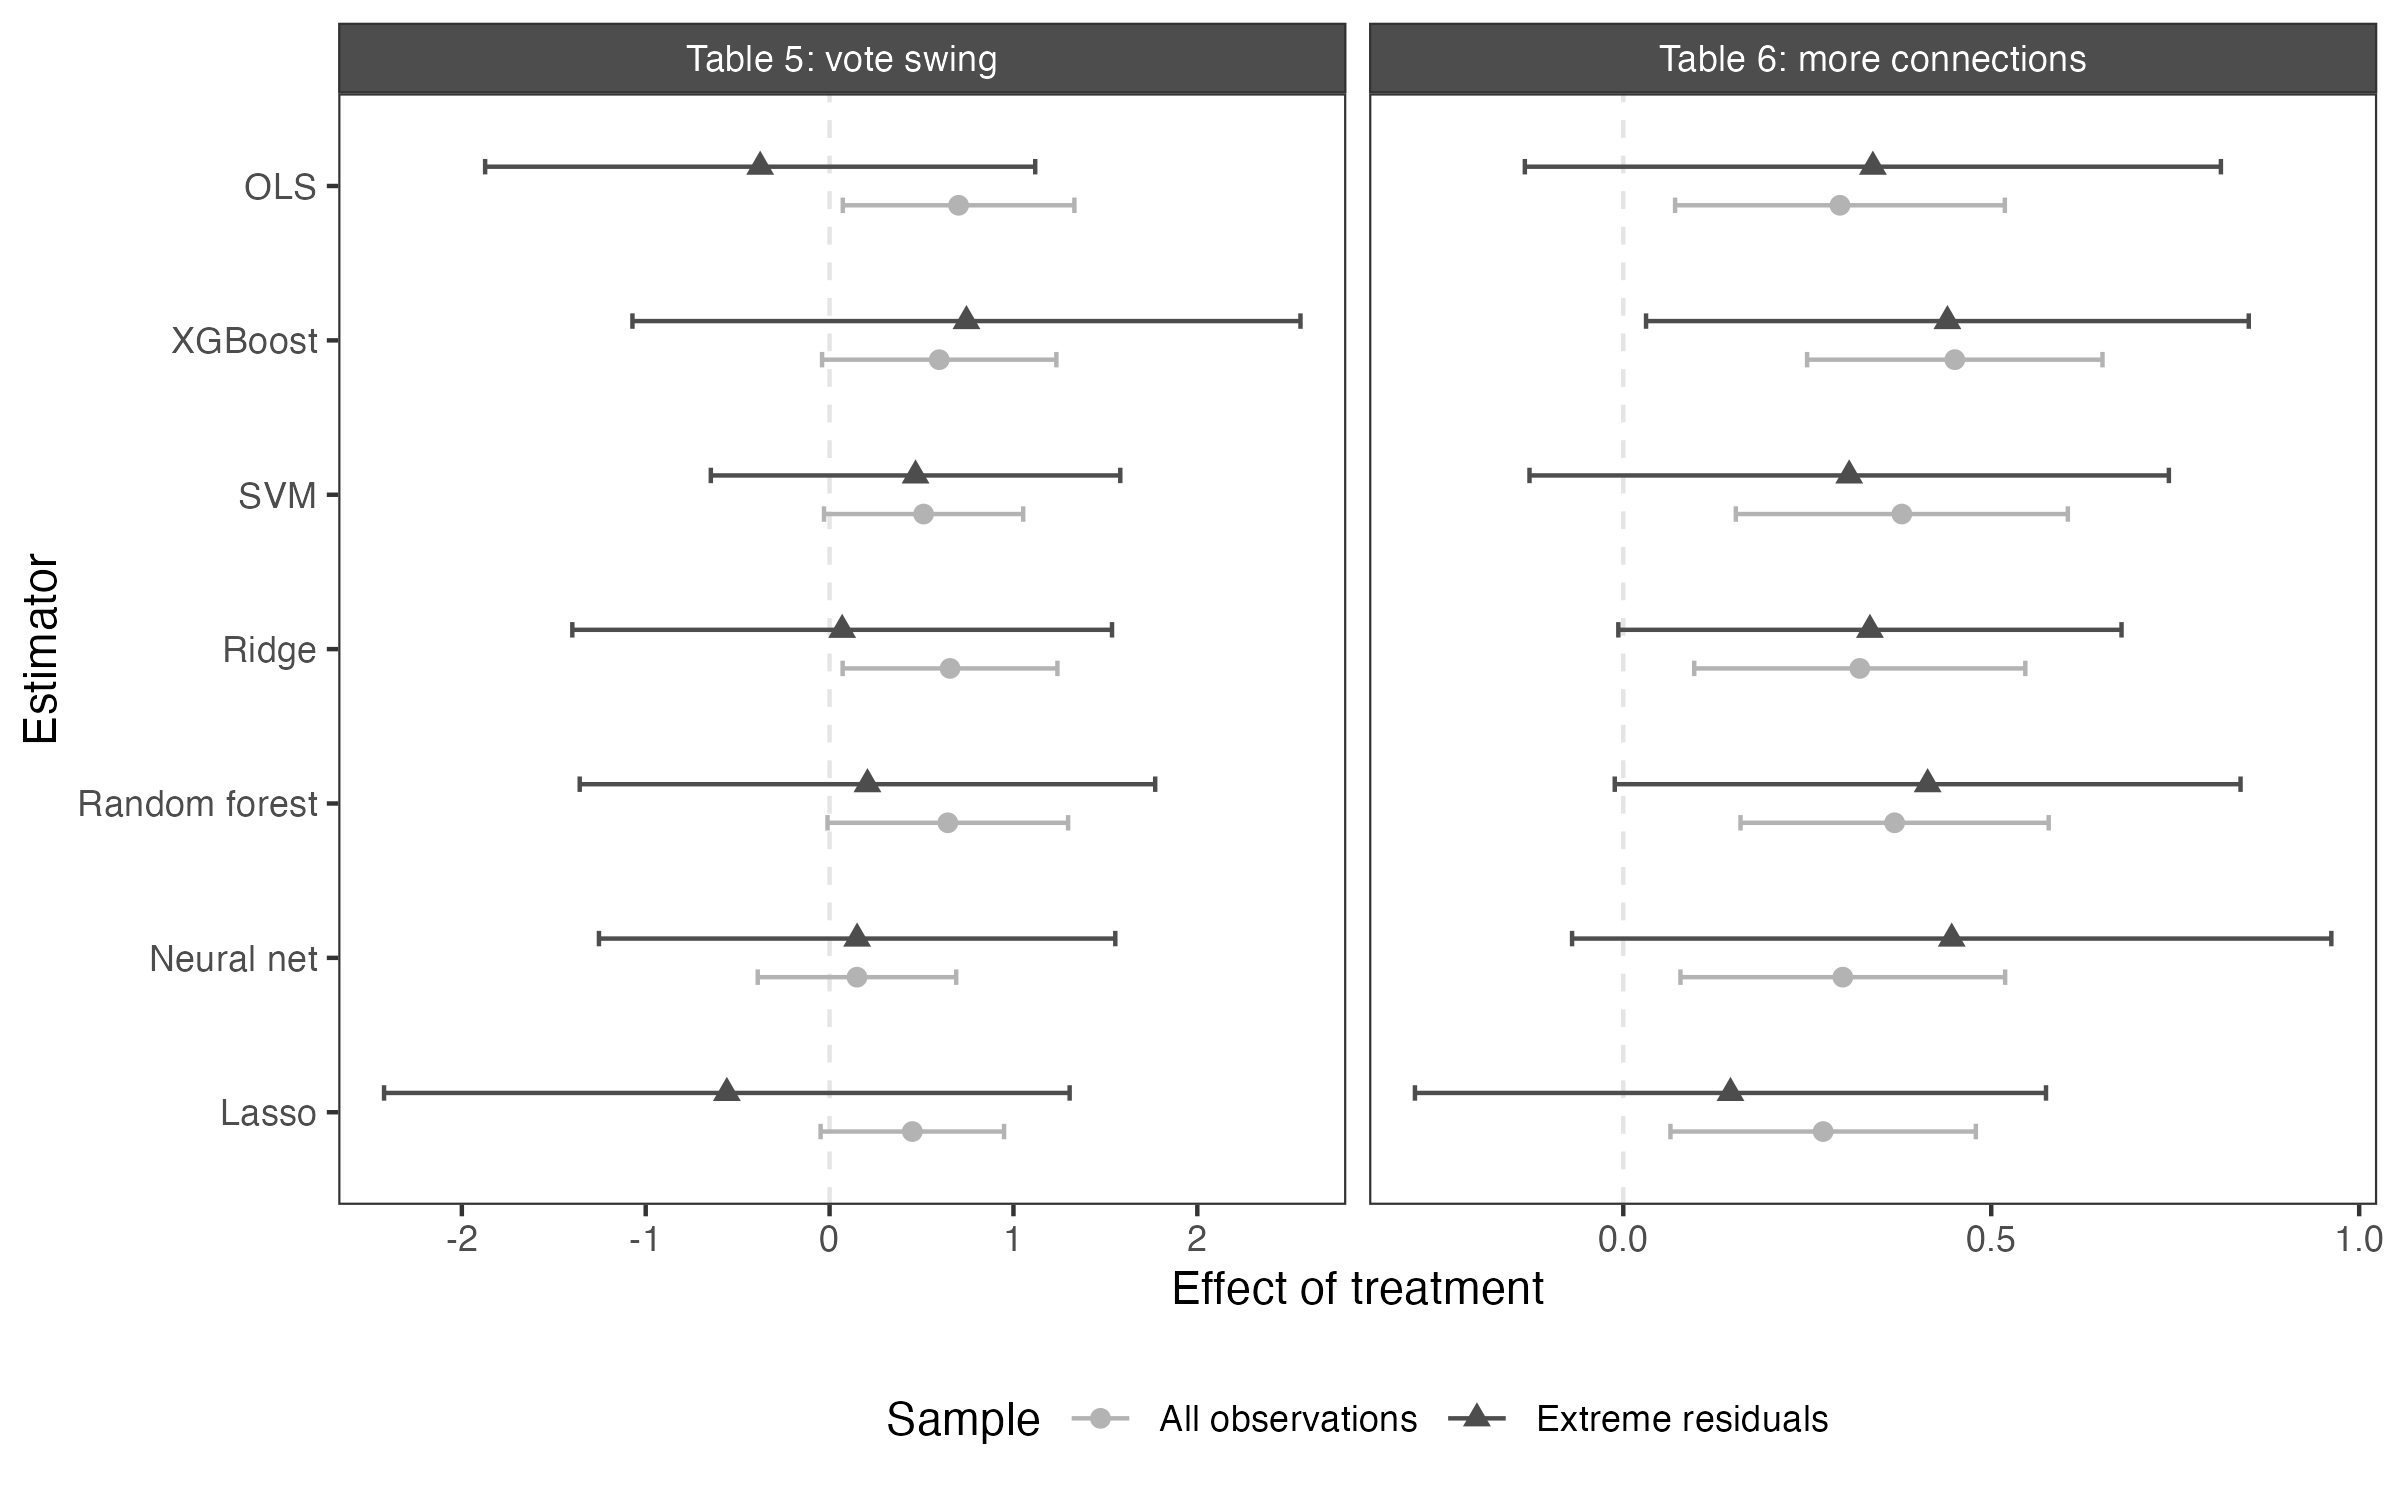
\includegraphics[height=0.6\textheight]{figures/observational_coefplot_predicted.png}
\end{figure}

\end{frame}


\section{Conclusions}

\begin{frame}[plain, label = two_dimensions]{Takeaways and Practical Advice}

\begin{itemize}
  \item \alert{\bf Learner choice matters} --- compare multiple learners.  \medskip \pause
    \item \alert{\bf Tuning parameters matter} --- more repetitions = more stable estimate; more folds = less overfitting.  \medskip \pause
  \item \alert{\bf Divergence across learners} indicates sensitivity to functional form.   \medskip \pause
  \item Differences with \alert{\bf OLS} suggest (1) \alert{treatment effect heterogeneity}, (2) \alert{nonlinearity}, or (3) \alert{limited overlap}.  \medskip \pause
  \item \alert{\bf Random assignment} ensures the propensity score model is correct, eliminating \alert{misspecification bias}. \medskip \pause
  \item \alert{\bf Binary vs.\ continuous} treatments rely on different estimators (\alert{AIPW} vs.\ \alert{PLR}).  \medskip \pause
  \item Standard DML assumes \alert{\bf i.i.d.}; clustering requires adjustments.  
 
\end{itemize}

\end{frame}



\section{Appendix}

\begin{frame}[plain,fragile,label=two_dimensions]{Code for DML with clustering}
\begin{minted}{r}
data_dml <- data |>
  # turn into data.table
  as.data.table() |>
  # create the DML data object
  DoubleMLClusterData$new(y_col = outcome,
                          d_cols = treatment,
                          x_cols = c(covariates, dummies),
                          cluster_cols = clusters)
# define learner as random forest
learner <- lrn("regr.ranger")
# obtain two clones of the learner
ml_l_sim <- learner$clone()
ml_m_sim <- learner$clone()
dml_object <- data_dml |>
  # specify the learners
  DoubleMLPLR$new(ml_l = ml_l_sim, ml_m = ml_m_sim,
                  # use 5-fold cross-fitting and 20 rounds
                  n_folds=5, n_rep=20)
# fit the model
dml_object$fit()
# extract the coefficients and standard errors
coefficients <- tibble(estimate = dml_object$coef, se = dml_object$se)
\end{minted}
\end{frame}


\end{document}